\section{1174077 - Alvan Alvanzah}
\subsection{Teori}
\begin{enumerate}

	\item Jelaskan apa itu klasifikasi teks, sertakan gambar ilustrasi buatan sendiri.
	\hfill\break
	Klasifikasi teks merupakan sebuah model yang biasa digunakan untuk untuk mengkategorikan sebuah teks ke dalam kelompok-kelompok yang lebih terorganisir. Jadi untuk setiap kalimat yang di masukan ke dalam mesin, mesin tersebut akan menjadikan setiap kata dari kalimat tersebut menjadi sebuah kolom. Untuk ilustrasinya bisa dilihat pada gambar berikut : 

	\begin{figure}[H]
	\centering
		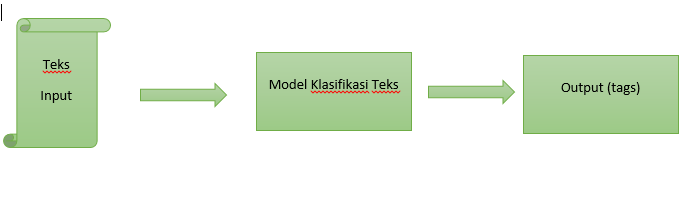
\includegraphics[width=4cm]{figures/1174077/4/materi/1.PNG}
		\caption{Klasifikasi teks.}
	\end{figure}

	\item Jelaskan mengapa hal ini bisa terjadi, klasifikasi bunga tidak bisa digunakan untuk machine learning, sertakan ilustrasi gambar sendiri.
	\hfill\break
	Karena machine learning tidak dapat menampilkan inputan sesuai dengan apa yang kita inputkan. Karena inputan tersebut serupa namun mesin memberikan output yang berbeda, biasanya output atau error ini disebut dengan istilah noise. Untuk contoh sederhananya misalkan kita inputkan salah satu label yang terdapat pada bunga, output yang dihasilkan oleh mesin tersebut ialah label yang lain. Itu dikarenakan bunga banyak jenis yang serupa namun tidak sama. Untuk ilustrasinya bisa dilihat pada gambar berikut : 

	\begin{figure}[H]
	\centering
		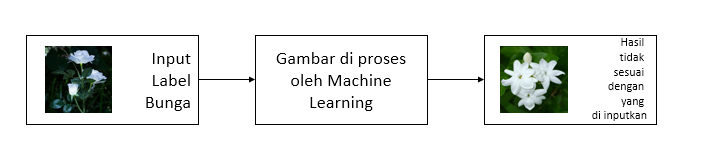
\includegraphics[width=4cm]{figures/1174077/4/materi/2.PNG}
		\caption{Klasifikasi Bunga.}
	\end{figure}
	
	\item Jelaskan bagaimana yang dimaksud dengan teknik pembelajaran mesin pada teks yang digunakan dan sertakan ilustrasi buatan sendiri.
	\hfill\break
	Teknik yang digunakan pada youtube salah satunya ialah keywords. Dengan keywords tersebut mesin dapat memberikan video sesuai dengan keyword yang kita inputkan pada kolom pencarian. Teknik pembelajarannya tergantung user memberikan input teks seperti apa, karena pada youtube itu sendiri akan menyesuaikan dengan apa yang biasa kita inputkan dan akan memfilter video secara otomatis sesuai dengan keyword yang biasa kita inputkan. Contoh ilustrasi sederhananya seperti berikut :

	\begin{figure}[H]
	\centering
		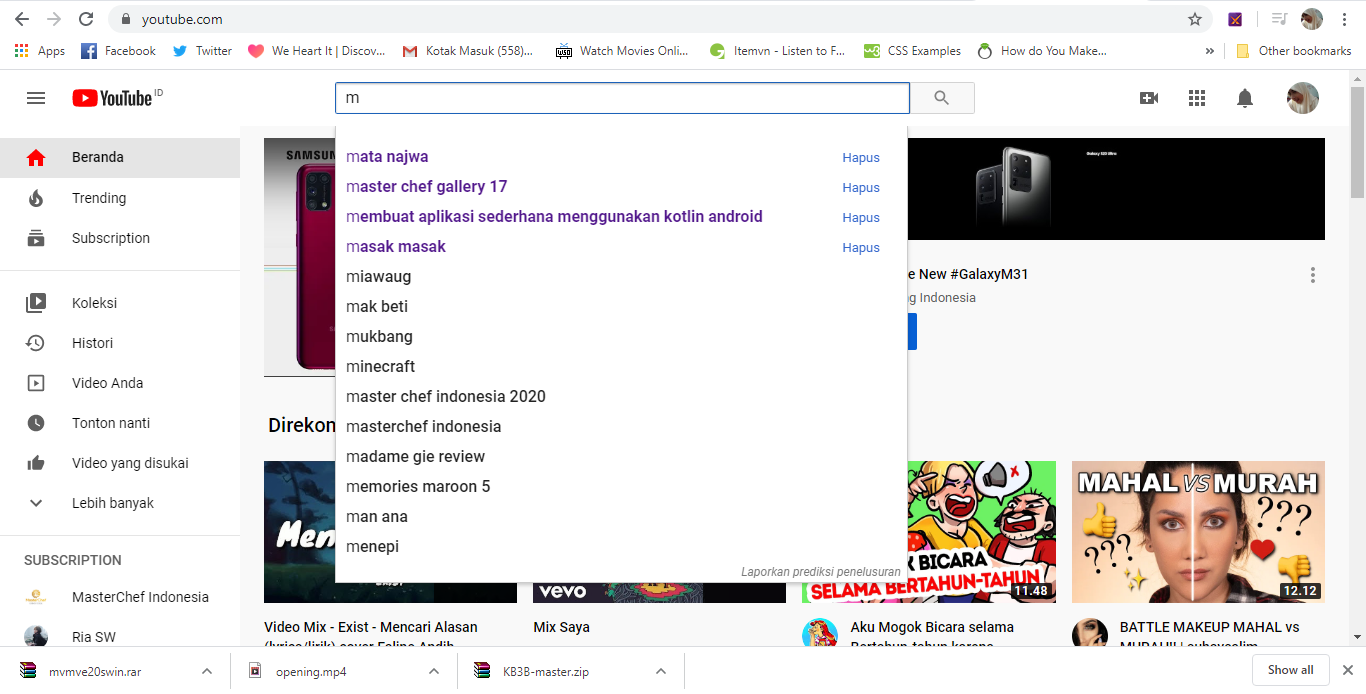
\includegraphics[width=4cm]{figures/1174077/4/materi/3.PNG}
		\caption{Klasifikasi teks Youtube.}
	\end{figure}

	\item Jelaskan apa yang dimaksud vektorisasi data.
	\hfill\break
	Vektorisasi data ialah suatu pemecahan atau pembagian data berupa teks, sebagai contoh terdapat 5 paragraf, data teks tersebut di pecah menjadi kalimat-kalimat yang lebih sederhana, lalu di pecah lagi menjadi kata untuk setiap kalimatnya. 

	\item Jelaskan apa yang dimaksud dengan bag of words dengan ilustrasi sendiri.
	\hfill\break
	Representasi penyederhanaan sebuah kalimat atau perhitungan setiap kata pada suatu kalimat dengan presentase berapa kali muncul kata tersebut untuk setiap kalimatnya. Contoh ilustrasi sederhananya seperti berikut : 

	\begin{figure}[H]
	\centering
		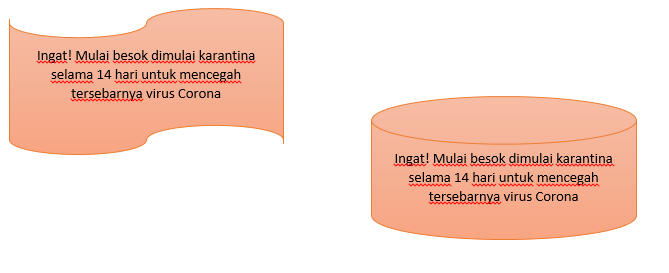
\includegraphics[width=4cm]{figures/1174077/4/materi/4.PNG}
		\caption{Bag of words.}
	\end{figure}

	\item Jelaskan apa yang dimaksud dengan TF-IDF.
	\hfill\break
	TF-IDF merupakan metode untuk menghitung bobot setiap kata pada suatu kalimat yang paling sering digunakan. TF-IDF ini akan menghitung nilai Term Frequency dan Inverse Document Frequency pada setiap kata dalam setiap kalimat yang muncul dengan diimbangi dengan jumlah dokumen dalam korpus yang mengandung kata. Contoh ilustrasi sederhananya seperti gambar berikut : 
	\end{enumerate}
	\begin{figure}[H]
	\centering
		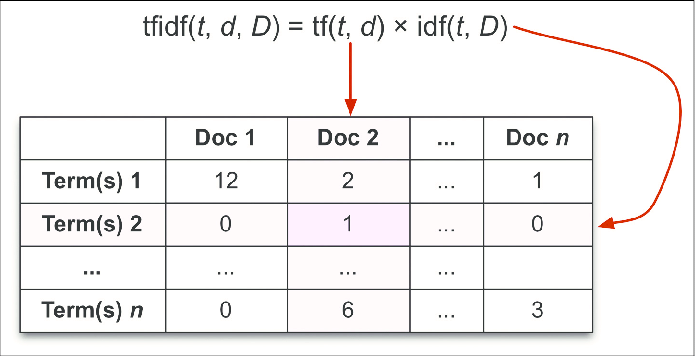
\includegraphics[width=4cm]{figures/1174077/4/materi/5.PNG}
		\caption{TF-IDF.}
	\end{figure}

\subsection{Praktek Program}
\begin{enumerate}
	\item Soal 1
	\hfill\break
	\lstinputlisting[firstline=8, lastline=10]{src/1174077/4/tugas4.py}
	Kode di atas digunakan untuk buat aplikasi sederhana menggunakan pandas dengan format csv sebanyak 500 baris, hasilnya ialah sebagai berikut : 
	\begin{figure}[H]
	\centering
		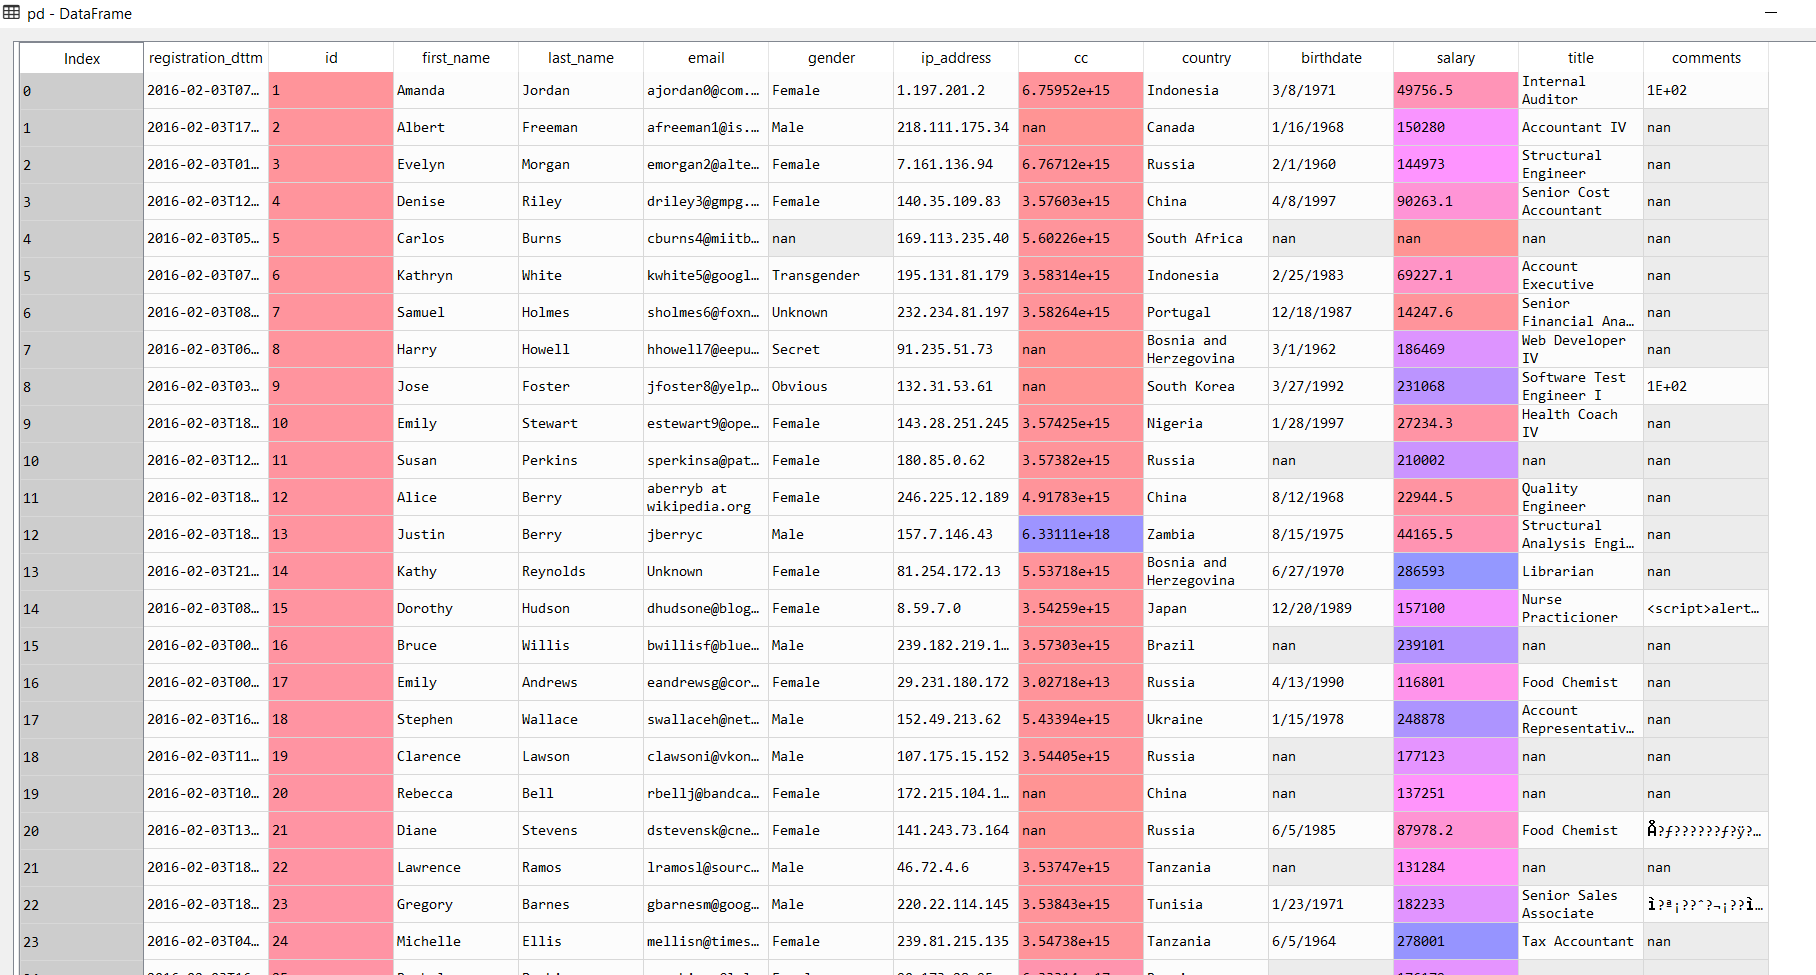
\includegraphics[width=4cm]{figures/1174077/4/materi/hasil1.PNG}
		\caption{Hasil Soal 1.}
	\end{figure}

	\item Soal 2
	\hfill\break
	\lstinputlisting[firstline=12, lastline=14]{src/1174077/4/tugas4.py}
	Kode di atas digunakan untuk memecah dataframe tersebut menjadi dua bagian yaitu 450 row pertama dan 50 row kedua. Hasilnya adalah sebagai berikut :
	\begin{figure}[H]
	\centering
		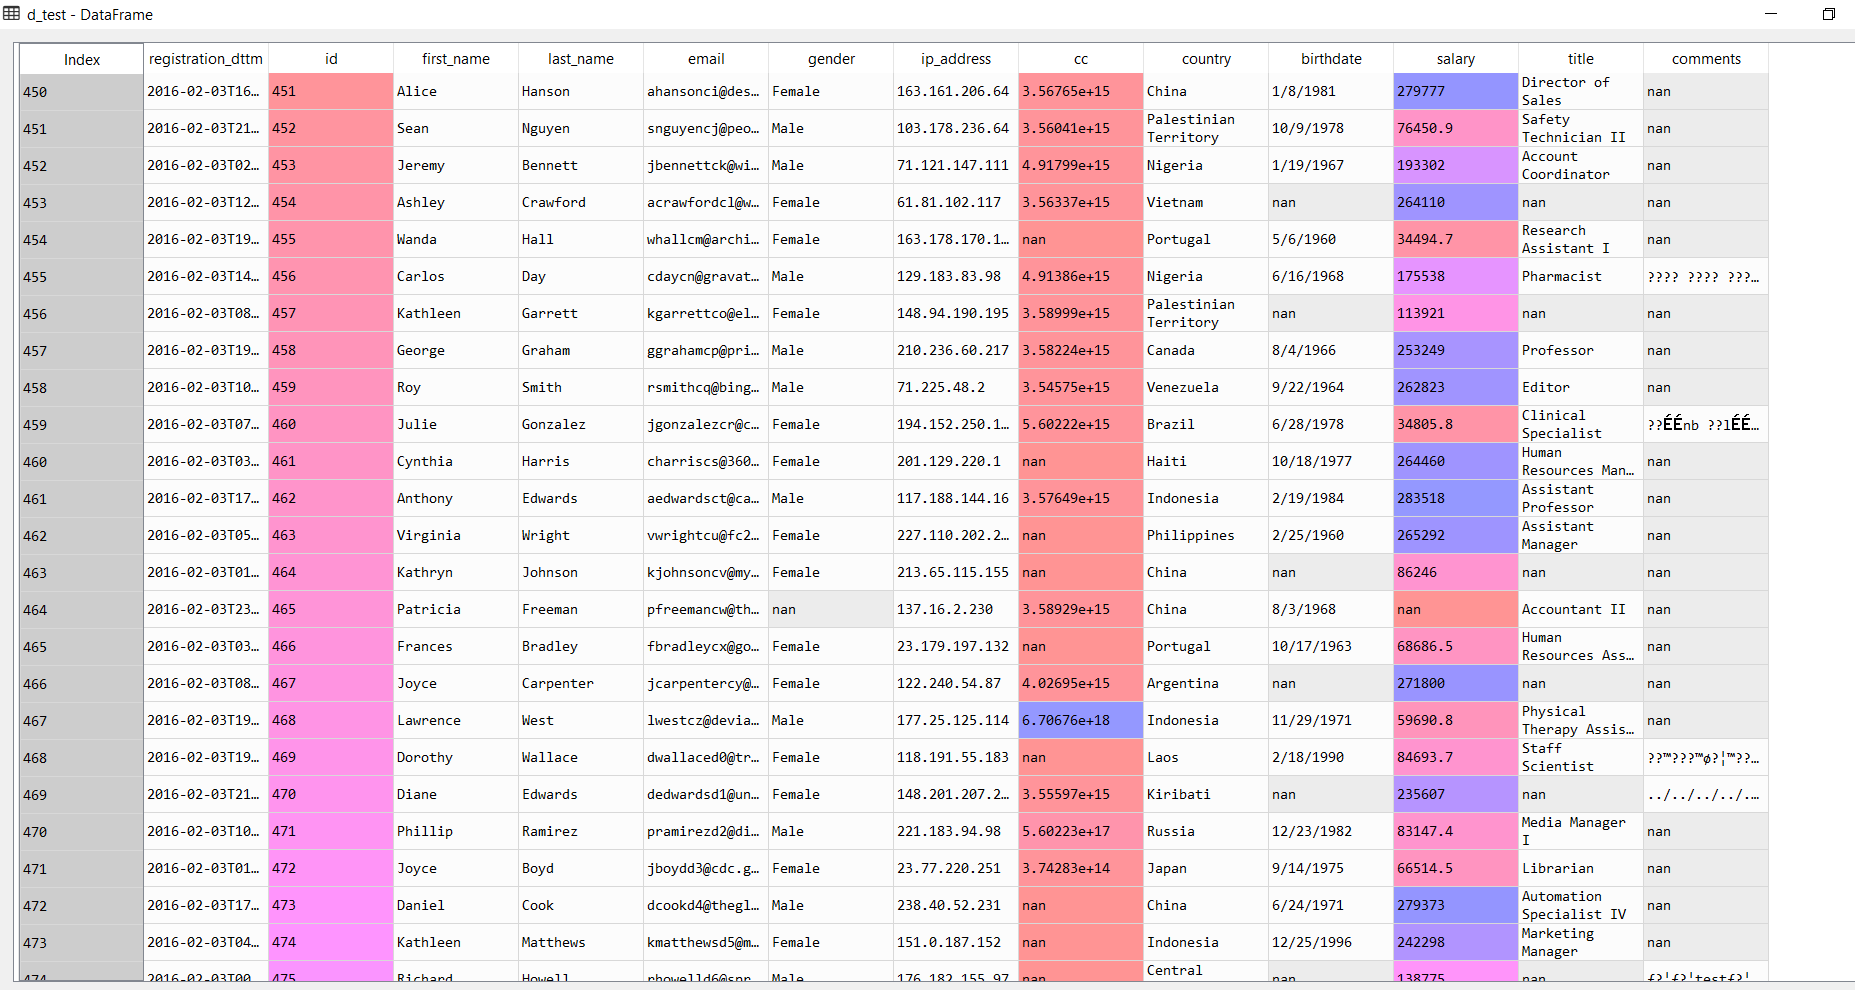
\includegraphics[width=4cm]{figures/1174077/4/materi/hasil21.PNG}
		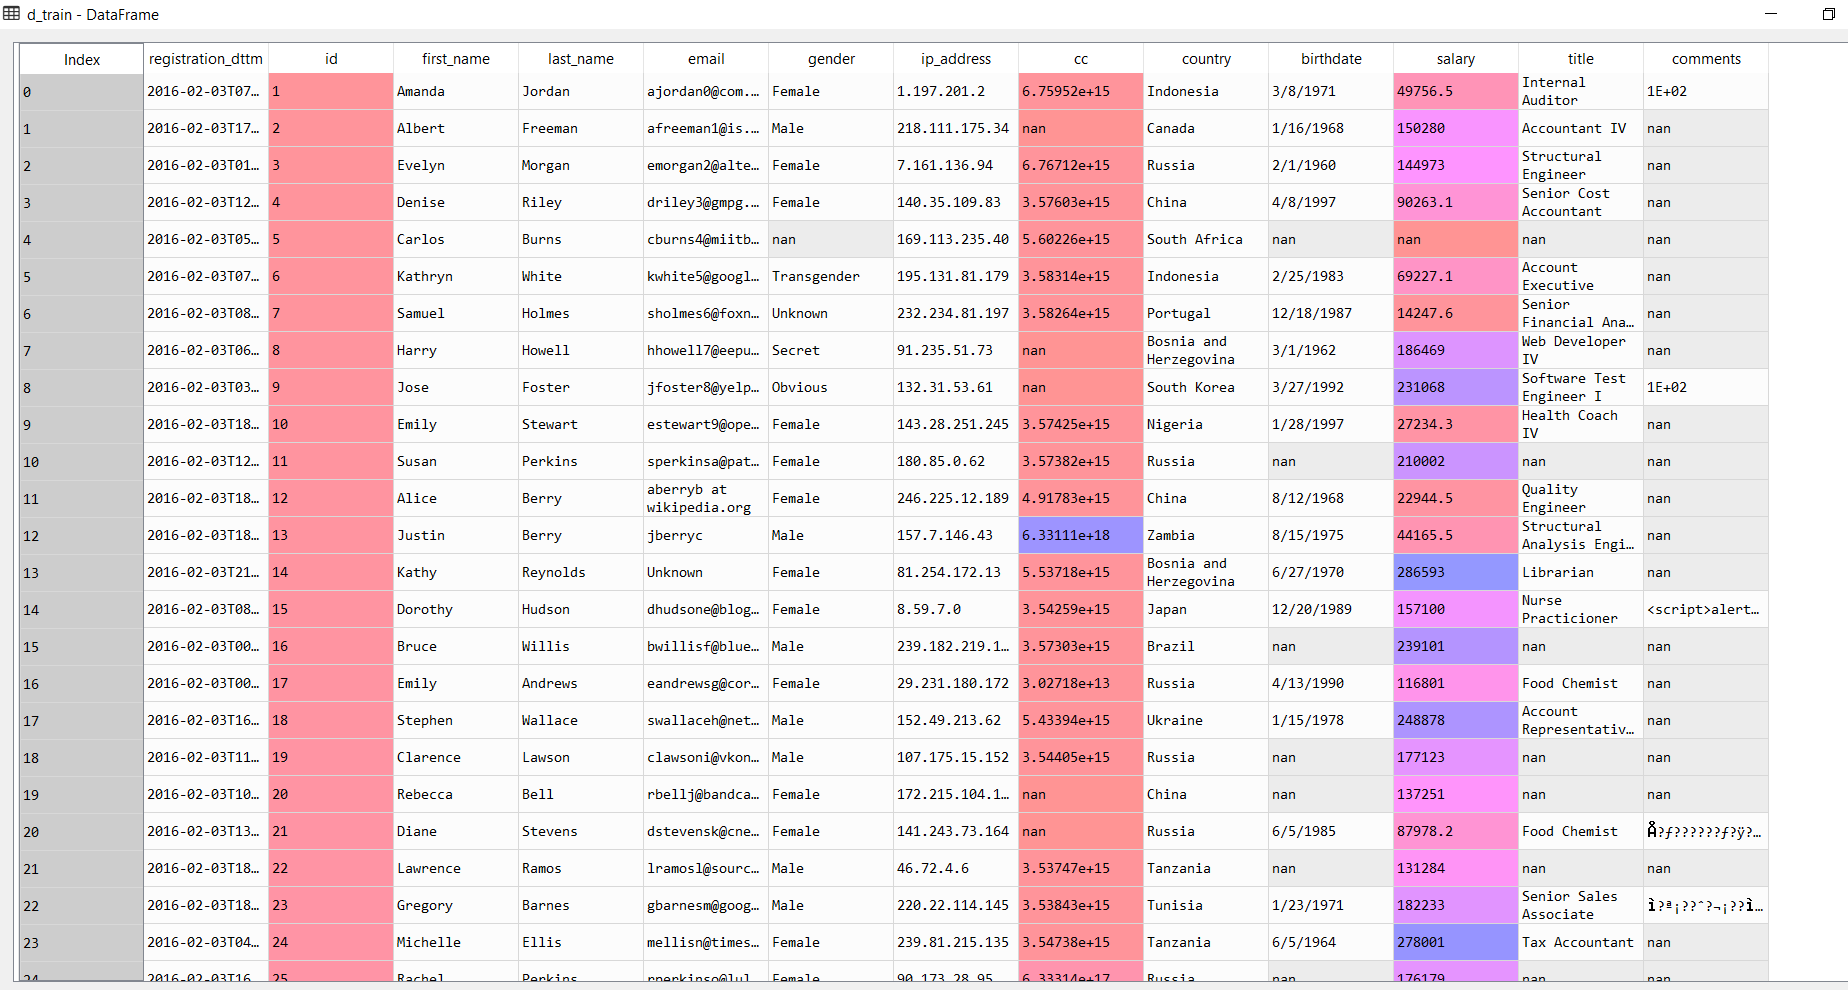
\includegraphics[width=4cm]{figures/1174077/4/materi/hasil22.PNG}
		\caption{Hasil Soal 2.}
	\end{figure}
	
	\item Soal 3
	\hfill\break
	\lstinputlisting[firstline=16, lastline=40]{src/1174077/4/tugas4.py}
	Dengan menggunakan 1174077 mod 4 adalah 1, yang artinya menggunakan dataset LMFAO. Hasilnya adalah sebagai berikut :
	\begin{figure}[H]
	\centering
		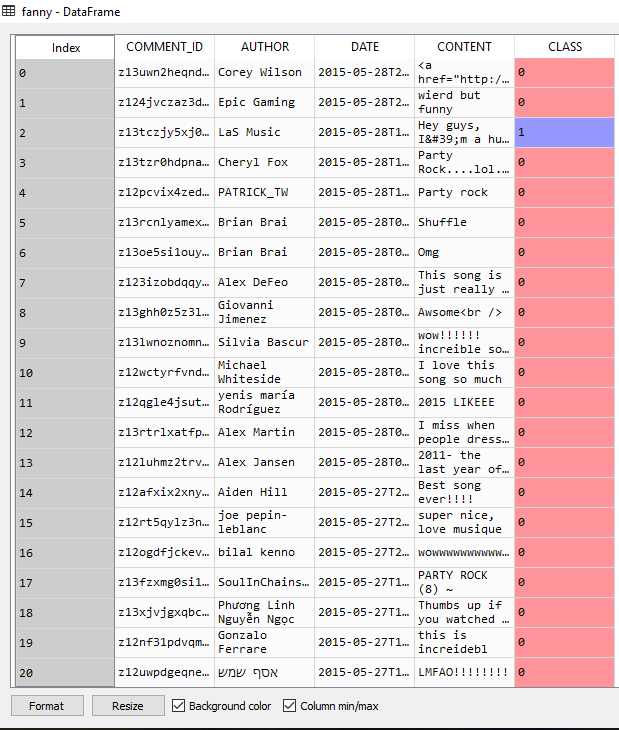
\includegraphics[width=4cm]{figures/1174077/4/materi/hasil31.PNG}
		\caption{Hasil Soal 3.}
	\end{figure}

	\item Soal 4
	\hfill\break
	\lstinputlisting[firstline=42, lastline=46]{src/1174077/4/tugas4.py}
	Klasifikasi dari data vektorisasi menggunakan klasifikasi Decision Tree. Hasilnya adalah sebagai berikut :
	\begin{figure}[H]
	\centering
		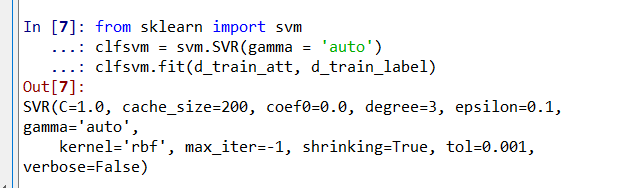
\includegraphics[width=4cm]{figures/1174077/4/materi/hasil4.PNG}
		\caption{Hasil Soal 4.}
	\end{figure}

	\item Soal 5
	\hfill\break
	\lstinputlisting[firstline=48, lastline=52]{src/1174077/4/tugas4.py}
	Plotlah confusion matrix dari praktik modul ini menggunakan matplotlib. Hasilnya adalah sebagai berikut :
	\begin{figure}[H]
	\centering
		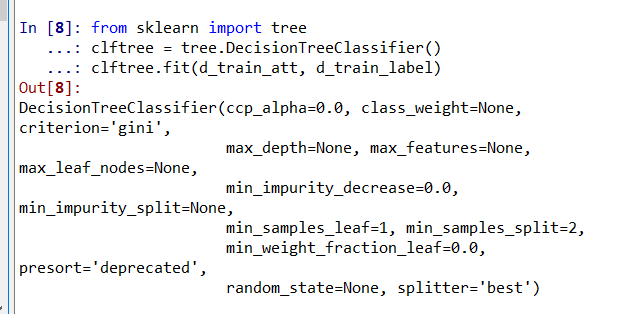
\includegraphics[width=4cm]{figures/1174077/4/materi/hasil5.PNG}
		\caption{Hasil Soal 5.}
	\end{figure}

	\item Soal 6
	\hfill\break
	\lstinputlisting[firstline=54, lastline=75]{src/1174077/4/tugas4.py}
	Menjalankan program cross validation. Hasilnya adalah sebagai berikut :
	\begin{figure}[H]
	\centering
		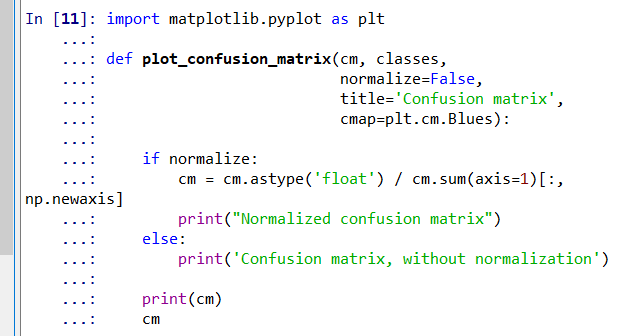
\includegraphics[width=4cm]{figures/1174077/4/materi/hasil6.PNG}
		\caption{Hasil Soal 6.}
	\end{figure}

	\item Soal 7
	\hfill\break
	\lstinputlisting[firstline=77, lastline=84]{src/1174077/4/tugas4.py}
	Tree.export graphviz merupakan fungsi yang menghasilkan representasi Graphviz dari decision tree, yang kemudian ditulis ke outfile.Disini akan menyimpan classifiernya, akan meng ekspor file student performance jika salah akan mengembalikan nilai fail. Hasilnya adalah sebagai berikut :
	\begin{figure}[H]
	\centering
		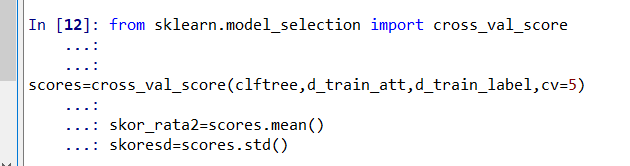
\includegraphics[width=4cm]{figures/1174077/4/materi/hasil7.PNG}
		\caption{Hasil Soal 7.}
	\end{figure}

	\item Soal 8
	\hfill\break
	\lstinputlisting[firstline=86, lastline=102]{src/1174077/4/tugas4.py}
	Buatlah program pengamatan komponen informasi. Jadi disini kita akan memprediksi nilai dari variabel test att dan test pass Hasilnya adalah sebagai berikut :
	\begin{figure}[H]
	\centering
		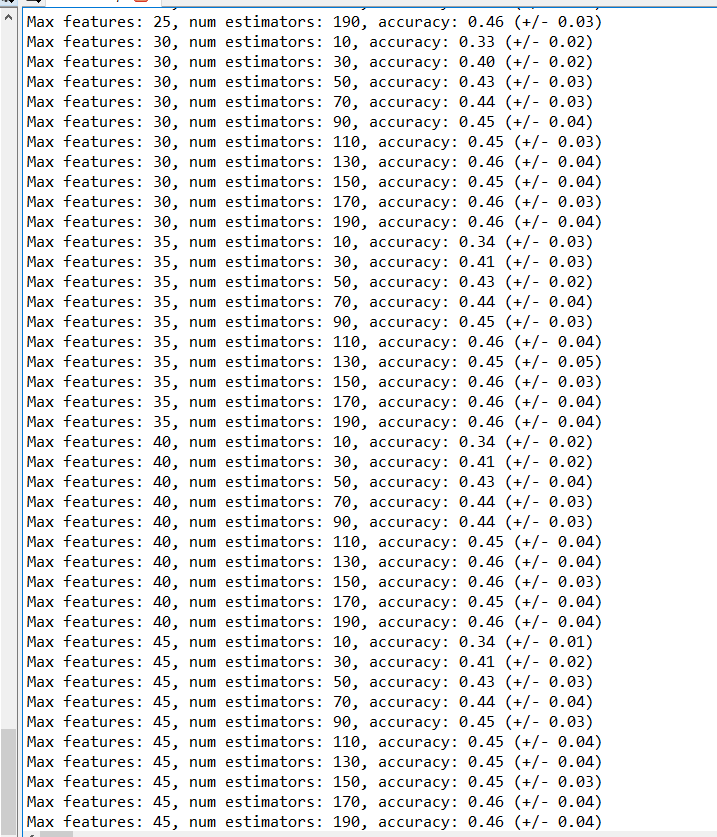
\includegraphics[width=4cm]{figures/1174077/4/materi/hasil8.PNG}
		\caption{Hasil Soal 8.}
	\end{figure}
\end{enumerate}

\subsection{Penanganan Error}
\begin{enumerate}
	\item ScreenShoot Error
	\begin{figure}[H]
		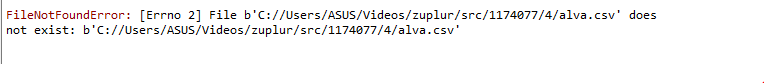
\includegraphics[width=4cm]{figures/1174077/4/error/1.PNG}
		\centering
		\caption{SyntaxError}
	\end{figure}
	\item Cara Penangan Error
	\begin{itemize}
		\item SyntaxError
		\hfill\break
		Dengan menyesuaikan letak file csv pada codingannya, sehingga dapat  di baca atau dipanggil file csvnya.
	\end{itemize}
\end{enumerate}

\subsection{Bukti Tidak Plagiat}
\begin{figure}[H]
\centering
	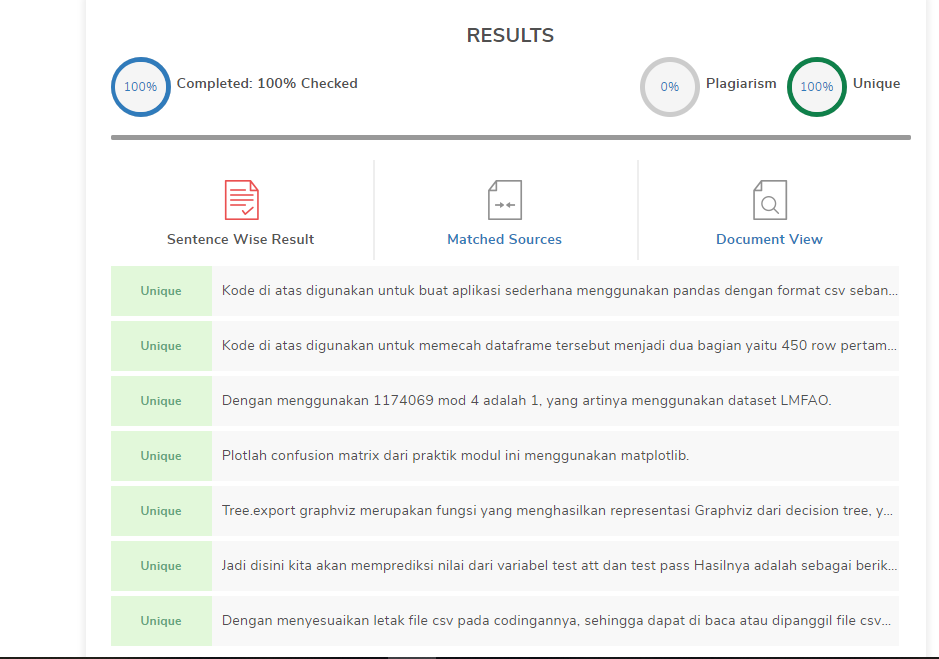
\includegraphics[width=4cm]{figures/1174077/4/buktiplagiat/1.PNG}
	\caption{Bukti Tidak Melakukan Plagiat Chapter 4}
\end{figure}

\subsection{Link Youtube}


